\documentclass[english,11pt]{article}

\usepackage[T1]{fontenc}
\usepackage[utf8]{inputenc}
\usepackage{hyperref}
\usepackage{graphicx}
\usepackage{babel}
\usepackage{color}
\usepackage{caption}
\usepackage{subcaption}
\usepackage{float}
\graphicspath{{./images/}}

\title{\textbf{Introduction to Neuroinformatics 1.0}
				\\Summary of the lectures 2012}
\author{Benjamin~Ellenberger}
\date{}
\begin{document}

\maketitle

\pagestyle{headings}
% The paper headers
\markboth{Neuroinformatics - Summary of the lecture}
{Neuroinformatics - Summary of the lecture}


\section{Lecture 1 - Neuroinformatics (Rodney Douglas)}
Introduction lecture, not much to learn yet.
\\
Aristotelian approach to 'Why?'
\begin{itemize}
\item Material cause
\item Effective cause
\item Formal cause
\item Final cause
\end{itemize}

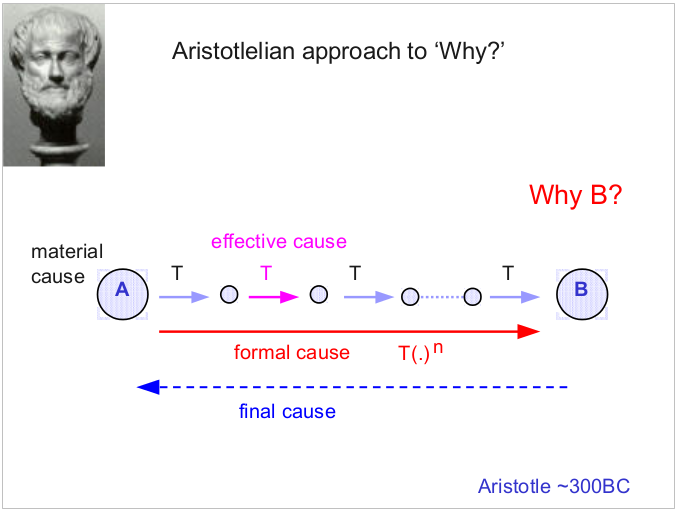
\includegraphics[width=0.7\textwidth]{aristothelian-why.png}

\section{Lecture 2 - Membrane Potentials (Rodney Douglas)}

\begin{figure}[h]
\begin{center}$
\begin{array}{cc}
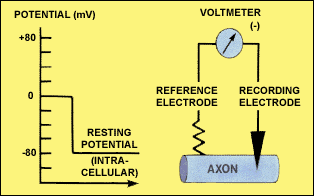
\includegraphics[width=0.5\textwidth]{voltage-source-in-membrane.png}

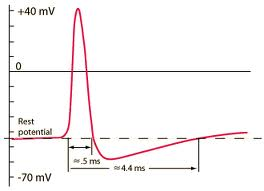
\includegraphics[width=0.5\textwidth]{voltage-source-in-membrane2.png}

\end{array}$
\end{center}
\end{figure}

The spike is the action potential caused by sodium ($Na^{2+}$) and changes in the membrane conductance. This shows that there is a voltage source in the membrane.

2 different types of neurons( prokaryotic, eukaryotic)
\begin{itemize}
\item Eukayotic cells differ in cell body components( Mitochondria, endoplasmatic reticulum, Golgi apparatus...)
\end{itemize}

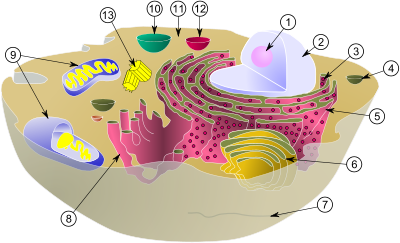
\includegraphics[width=0.8\textwidth]{subcellular-contents.png}

Typical animal (eukaryotic)
cell subcellular components:
\begin{enumerate}
\item nucleolus
\item nucleus
\item ribosome
\item vesicle
\item rough endoplasmic reticulum
\item Golgi apparatus
\item Cytoskeleton
\item smooth endoplasmic reticulum
\item mitochondria
\item vacuole
\item cytoplasm
\item lysosome
\item centrioles within centrosome
\end{enumerate}

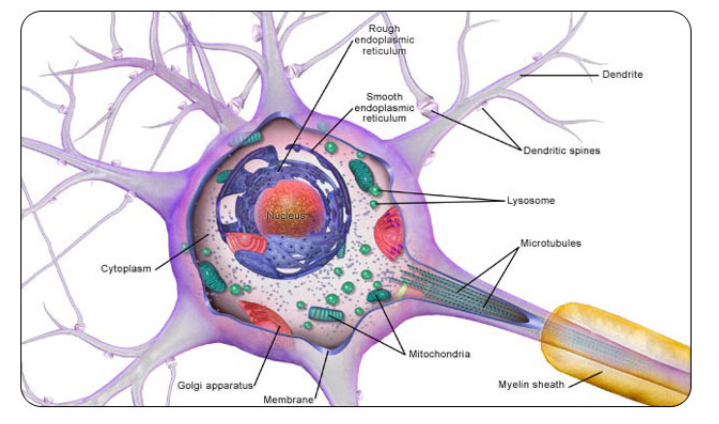
\includegraphics[width=\textwidth]{neuron.png}



\begin{figure}[h]
\begin{center}
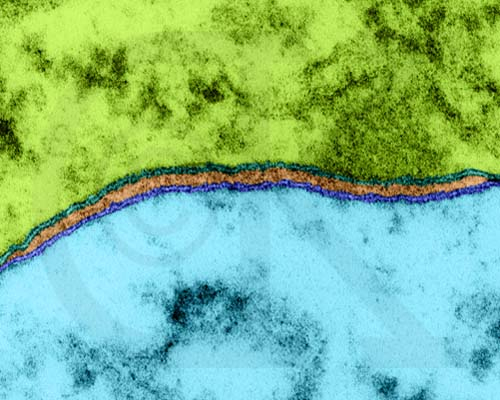
\includegraphics[width=0.6\textwidth]{bilayer.png}
\end{center}
\caption{The membrane bilayer}
\end{figure}



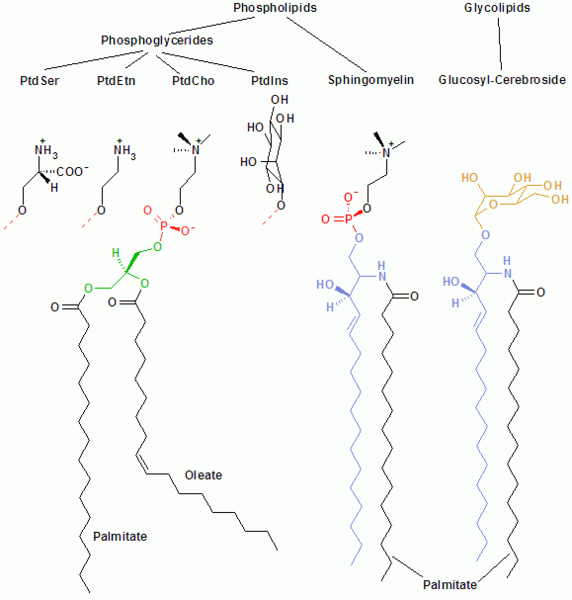
\includegraphics[width=0.7\textwidth]{charged-and-uncharged.png}\\
The bilayer is built out of those molecules whereas the charged sides align (such as the one with $N^{+}H_{3}$ and the uncharged ends align such as the long CH chain. The uncharged ends are hydrophobic).\\

ECS (Extra cellular solution)\\
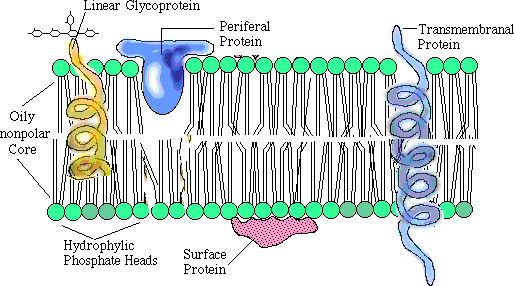
\includegraphics[width=\textwidth]{bilayer-closeup.png}\\
ICS (Intra cellular solution)\\
Transmembranal proteines play an important role as they have charged ends(phosphate heads) and uncharged bodies and therefore fit inside of the membrane as it aligns with the uncharged inner part of the membrane and with the outer charged parts.\\

2 basic mechanisms for the membrane potential:
\begin{itemize}
\item Gibbs-Donan equilibrium (Causes asymmetry across membrane)
\item Active mechanisms($Na^+$/$K^+$-Pump from ECF to ICF)
\end{itemize}

\subsection{Concentrations across the membrane}

\begin{tabular}{ l | c | r }
 -	& ICF & ECF \\
  $Na^+$(Sodium) & - & + \\
  $K^+$(Potassium) & + & - \\
  $Cl^-$(Chlorine) & + & - \\
  $Ca^{2+}$(Calcium) & x & (+) \\
  Large Anions(not passing membrane) & + & (-) \\
\end{tabular}

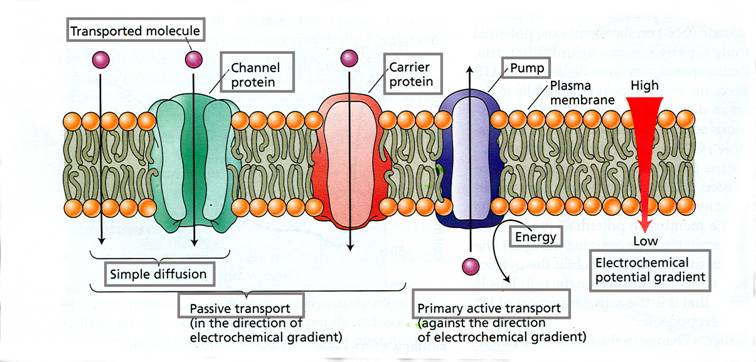
\includegraphics[width=\textwidth]{bilayer-closeup2.png}
There is a concentration gradient top-down from high concentration to low concentration. The pump uses ATP to build up the gradient if it is released.

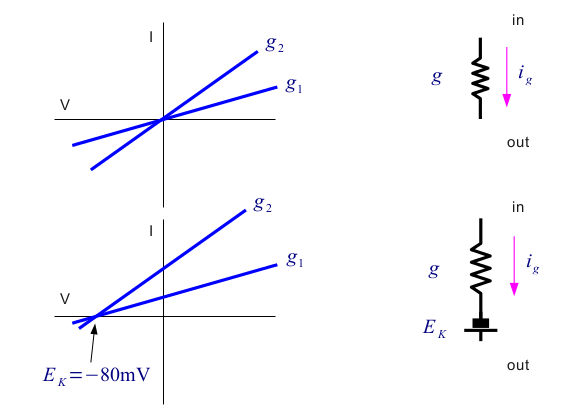
\includegraphics[width=\textwidth]{different-conductors.png}

The function of conduction is approximative linear and reaches $E_k~=~-80mV$ at the point of no current.

\subsection{Fick's Law of diffusion}
$J_{diff} = -D \frac{\delta[C]}{\delta x}$ (Concentration gradient)\\
$ICF \rightarrow ECF$\\

\begin{itemize}
\item J Diffusion flux ($\frac{molecules}{sec \cdot cm^2}$)
\item D Diffusion coefficient ($\frac{cm^2}{sec}$)
\item $[C]$ Concentration of species ($\frac{molecules}{cm^3}$)
\end{itemize}

\subsection{Ohm's law of drift}
$J_{drift} = \delta_{el}E = -\mu z [C] \frac{\delta V}{\delta x}$ (Voltage gradient)\\
$ICF \leftarrow ECF$\\

\begin{itemize}
\item J Drift flux ($\frac{molecules}{sec \cdot cm^2}$)
\item $\delta_{el}$ Electrical conductivity ($\frac{molecules}{V \cdot sec \cdot cm}$)
\item $E=-\frac{\delta V}{\delta x}$ Electric field ($\frac{V}{cm}$)
\item V Electrical potential
\item $\mu$ Mobility of species ($\frac{cm^2}{V \cdot sec}$)
\item z Valence of ion (dimensionless)
\item $[C]$ Concentration of species ($\frac{molecules}{cm^3}$)
\end{itemize}

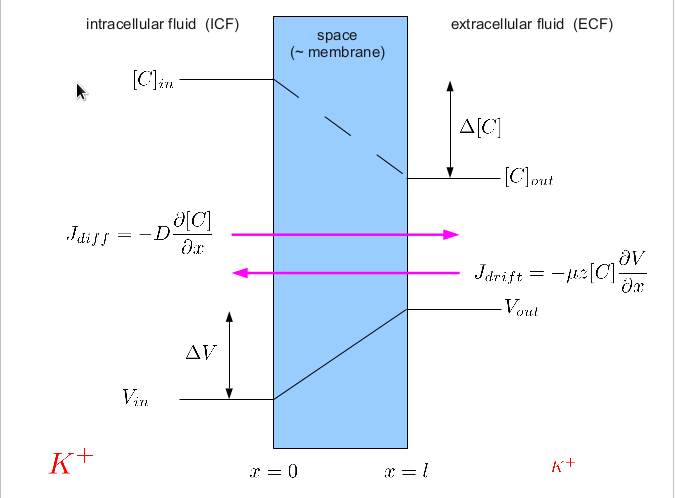
\includegraphics[width=\textwidth]{fluid-equations.png}

\subsection{Einstein's relation between diffusion and mobility}
Diffusion and drift are additive\\
$D = \frac{k \cdot T}{q} \mu$

\begin{itemize}
\item k Boltzmann's constant ($1.38 \times 10^{-23} \frac{Joule}{K}$)
\item T Absolute Temperature (K)
\item q Charge of the molecule (Coulombs)
\end{itemize}

\subsection{Nernst-Planck equation}
Substitues part of Einstein's formula
$J = J_{drift} + J_{diff} = -\mu z [C] \frac{\delta V}{\delta x} -D \frac{\delta[C]}{\delta x}$\\

Divided by Avogadro to obtain molar form, J scaled by zF to obtain molar charge\\

$I = J \cdot zF = -(\mu z^2 F [C] \frac{\delta V}{\delta x} +uzRT \frac{\delta[C]}{\delta x})$\\

at $37^\circ C \rightarrow -60 mV$

\begin{itemize}
\item R Universal gas constant ($8.3144 \frac{J}{mol \cdot K}$)
\item F Faraday constant ($ 96500 \frac{C}{mol}$)
\item u Molar mobility ($\frac{cm^2}{V \cdot sec \cdot mol}$)
\end{itemize}

\subsection{Goldman-Hodgkin-Katz equation (GHK-Voltage equation)}

$\Delta V = \frac{RT}{F} ln(\frac{P_K[K^+]_{out} + P_{Na}[Na^+]_{out} + P_{Cl}[Cl^{-}]_{in}}{P_K[K^+]_{in} + P_{Na}[Na^+]_{in} + P_{Cl}[Cl^{-}]_{out}})$

This is only for static situations but gives us a sense of how it is actually working.
Basic assumptions:
\begin{itemize}
\item Ion flux obeys Nernst/Planck equation
\item Ions move across membrane independently (no interaction)
\item Electric field in the membrane is constant $E = -\frac{\delta V}{\delta x} = - \frac{\Delta V}{l}$
\end{itemize}
\subsection{Permeability}

$J = -P\Delta[C]$\\
$ D^* = \mu^* \frac{kT}{q} = \mu^* \frac{RT}{F}$\\
$P = \frac{\beta D^*}{l} = \frac{\beta \mu^* RT}{lF}$\\

\begin{itemize}
\item $\beta$  Water-membrane partition coefficient for ion i
\item $\mu^*$ Mobility of ion i within the membrane
\item $D^*$ Diffusion coefficient within membrane
\end{itemize}



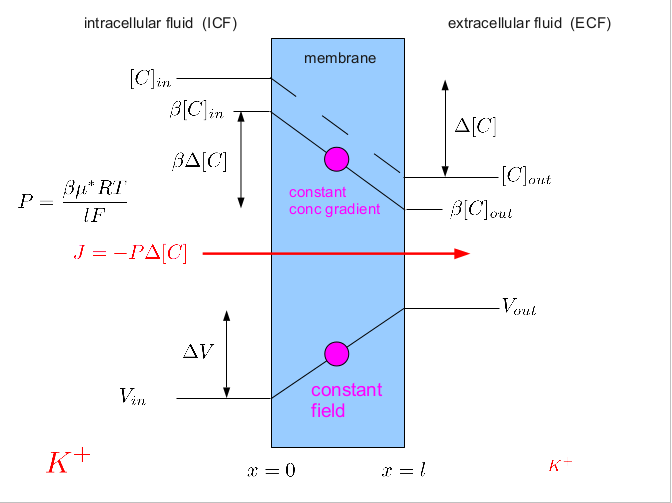
\includegraphics[width=\textwidth]{fluid-equations2.png}


\section{Lecture 3 - Passive (Cable) Membrane Properties (Rodney Douglas}

\begin{itemize}
\item $J_{diff}$ and $J_{drift}$ are in an equilibrium during the resting potential
\item Resting potential is due to $K^+$ concentration
\item GHK-equation $\Delta V = $ Difference in Potential across the membrane
\item if $P(Permeability) = 1 \rightarrow Nernst-equation$
\end{itemize}
\subsection{Ohmic model of biological membrane}
\begin{itemize}
\item 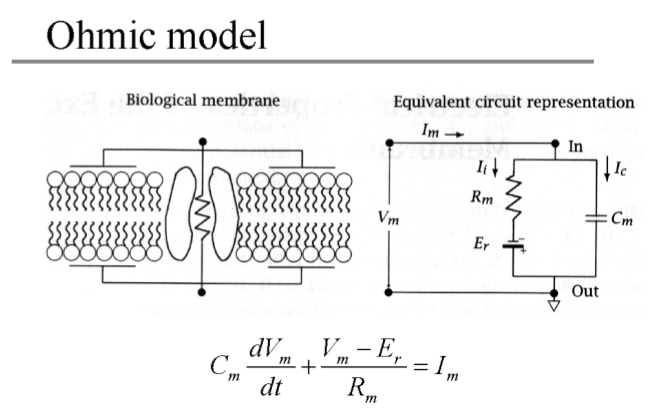
\includegraphics[width=\textwidth]{ohmic-model.png}\\
The conductor indicates the temporale dynamicity\\
Conductance $G = \frac{Current~I}{Voltage~U} = \frac{1}{Resistance~R}$ 
\item $I_c + I_o = I_m$
\item If $\frac{\delta V_m}{\delta t} = 0 \rightarrow$ membrane is at rest
\item Changing the permeability of the membrane results in changable conductance g in membrane $\rightarrow$ over time.
\item
\begin{figure}[H]
        \centering
        \begin{subfigure}[b]{0.5\textwidth}
                \centering
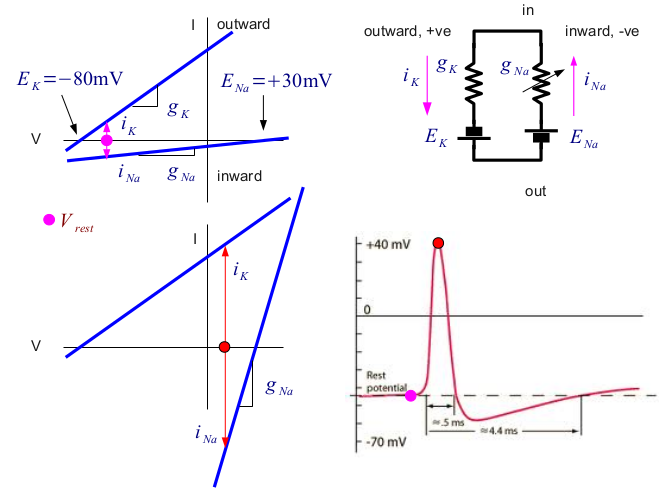
\includegraphics[width=\textwidth]{ohmic-model2.png}
        \end{subfigure}%
        ~
        \begin{subfigure}[b]{0.5\textwidth}
                \centering
				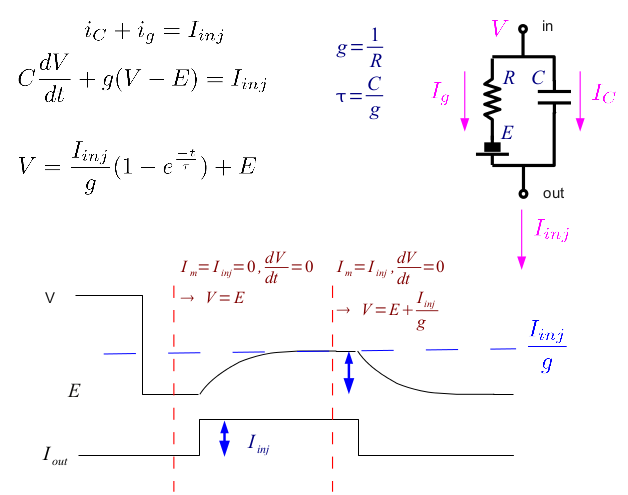
\includegraphics[width=\textwidth]{ohmic-model3.png}
        \end{subfigure}
\end{figure}

\end{itemize}
\subsection{Electrical nature of the membrane}
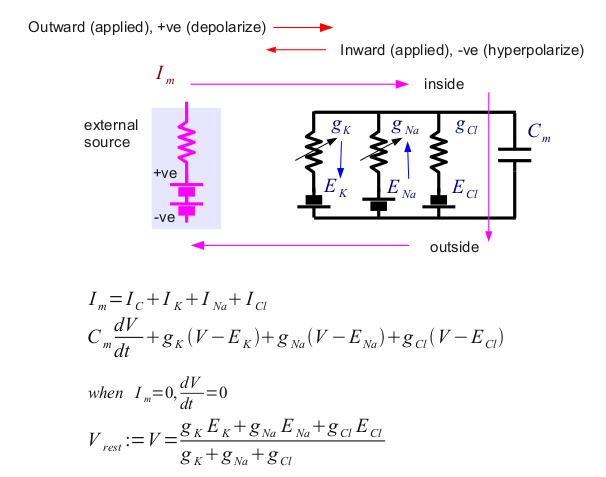
\includegraphics[width=0.5\textwidth]{electrical-membrane.png}
\begin{itemize}
\item Typical values for electrical properties of membranes:
\item Capacitance(Cell of $20\mu m$ diameter: $c_m =C_m \cdot A = 1\frac{\mu F}{cm^2} \cdot 10^{-5} \approx 10 pF$\\
Resistance:$r_m = \frac{R_m}{A} = \frac{10k\Omega\cdot cm^2}{10^{-5}} \approx 1000 M\Omega$\\
Time constant($\mu F \cdot M\Omega = sec$): $\tau_m = c_m r_m = \frac{R_m}{A}\cdot C_m A = R_m C_m \approx 10^{-6} \mu F \cdot 10^4\Omega = 10msec$
\item Membrane behaves like a resistance network\\
Current leaks out through membrane resistance\\
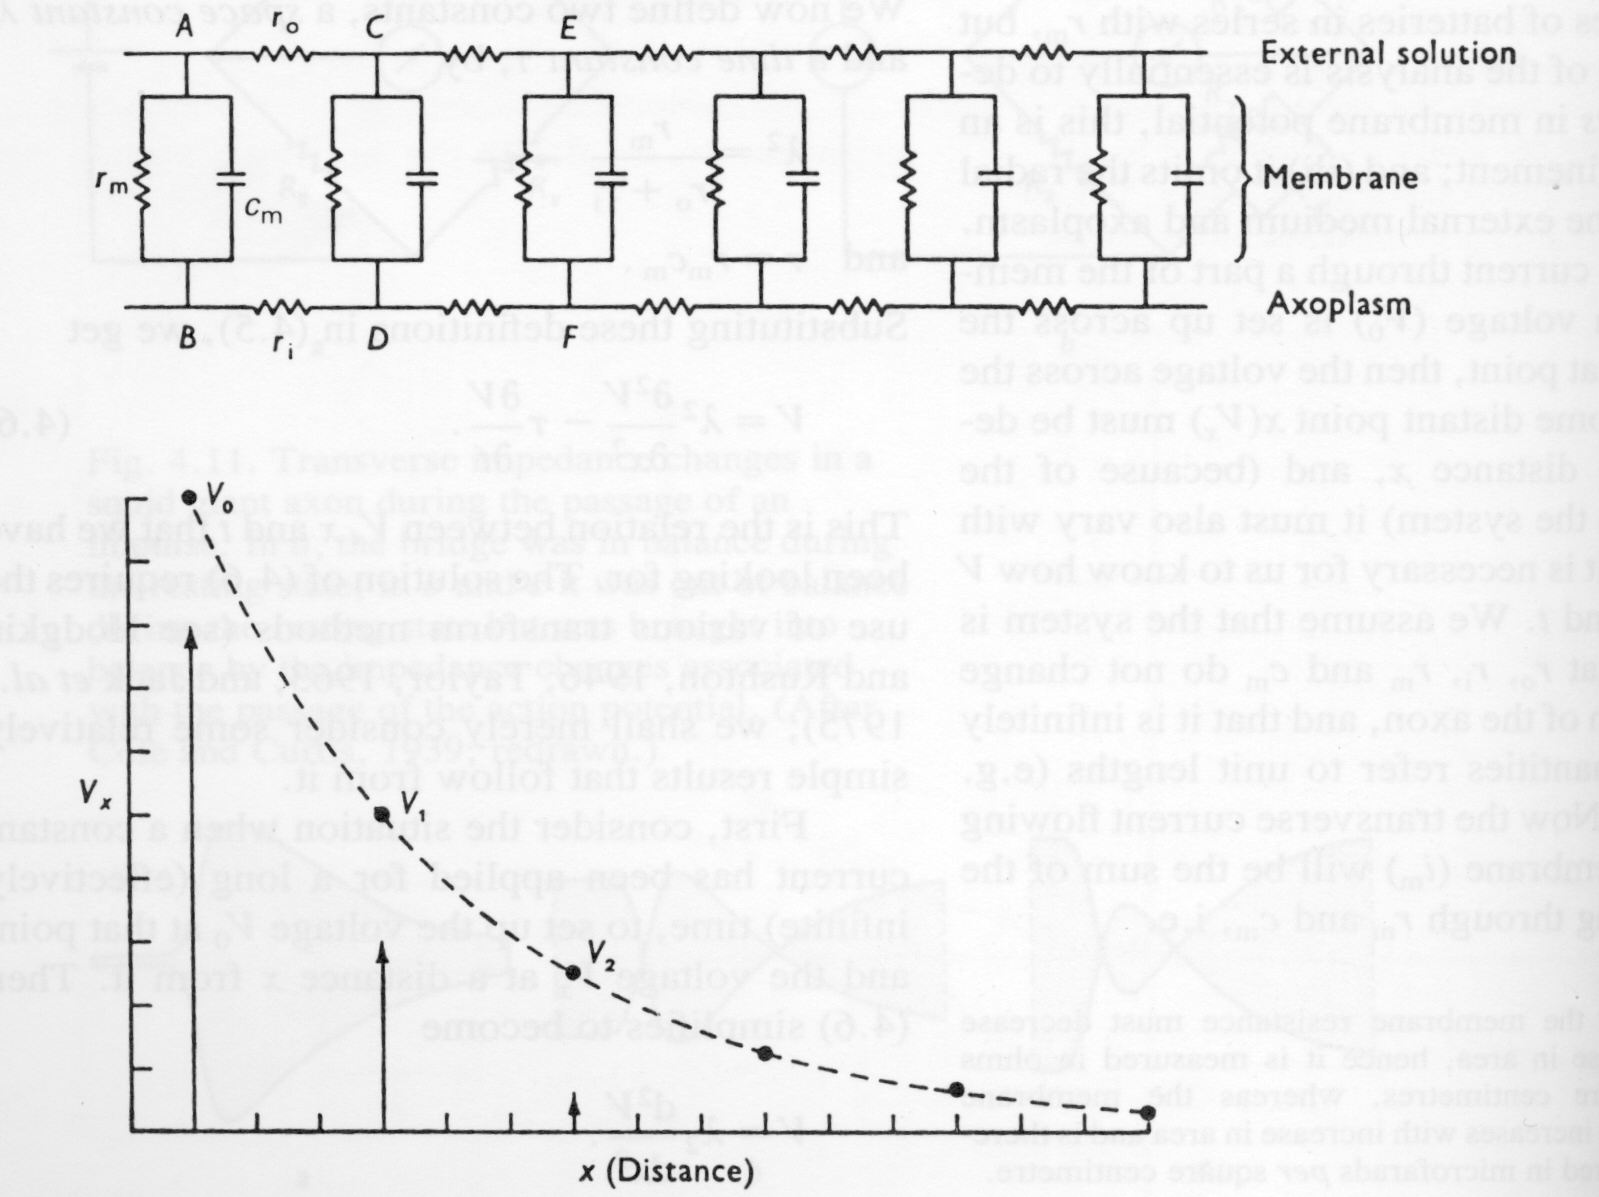
\includegraphics[width=0.6\textwidth]{membrane-leakage.png}\\
Voltage leakage is rising exponentially. 4 decay constants leads to $\approx 0 V$
\end{itemize}

\subsection{The cable equation}
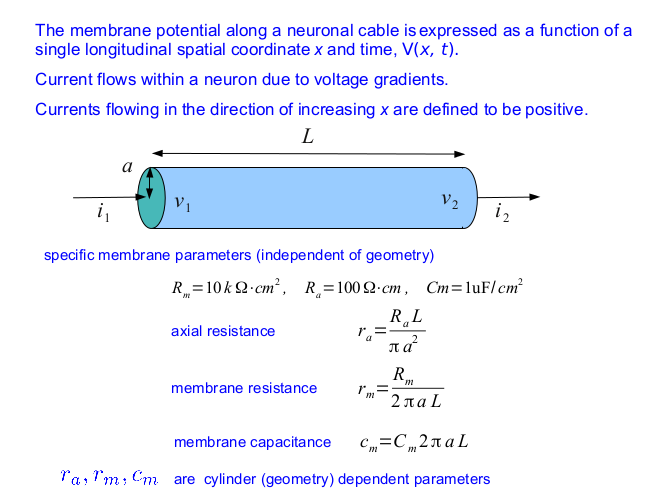
\includegraphics[width=0.9\textwidth]{cable-equation1.png}
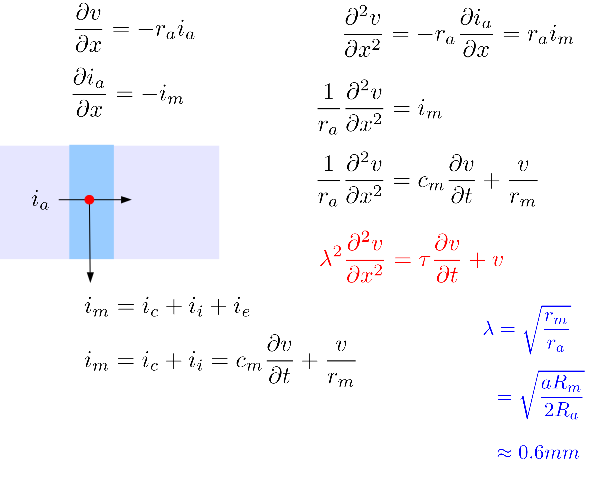
\includegraphics[width=0.9\textwidth]{cable-equation2.png}
$\tau$ = time constant\\
$\lambda$ = space constant for $R_m$ and $R_a$ of this cable.\\
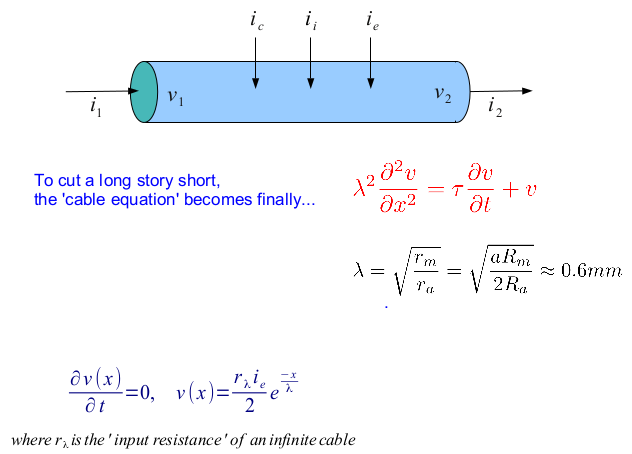
\includegraphics[width=\textwidth]{cable-equation3.png}
$\lambda = 0.6mm$ means no signal left after $0.6mm$\\
$\rightarrow$ Increasing $R_m$ of the cable increases $\lambda$\\
$\rightarrow$ Increasing diameter of the cable increases $\lambda$

\subsection{From exercises:Electric laws}
\begin{itemize}
\item Kirchhoff's Current Law (KCL): The sum of all currents entering and leaving any node in a circuit is not zero.
\item Kirchhoff's Voltage Law (KVL): The sum of all voltages around a closed loop is zero.
\item Ohm's Law: $V = I \cdot R$
\end{itemize}

\section{Lecture 4 - Action Potentials (Rodney Douglas)}
\begin{itemize}
\item Voltage Clamp experiment\\
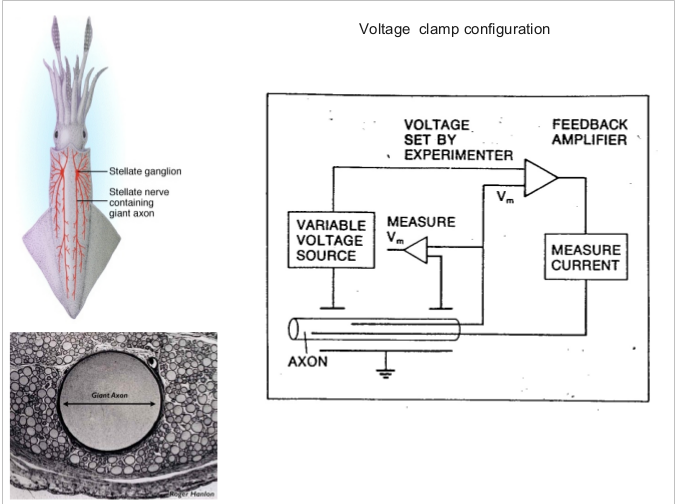
\includegraphics[width=\textwidth]{voltage-clamp-configuration.png}
\item With negative feedback circuit
\item Command voltage is set by the experimenter, the feedback circuit holds the voltage constant.
\item The voltage clamp allows the membrane voltage to be manipulated independently of ionic currents, allowing the current-voltage relationships of membrane channels to be studied.\\
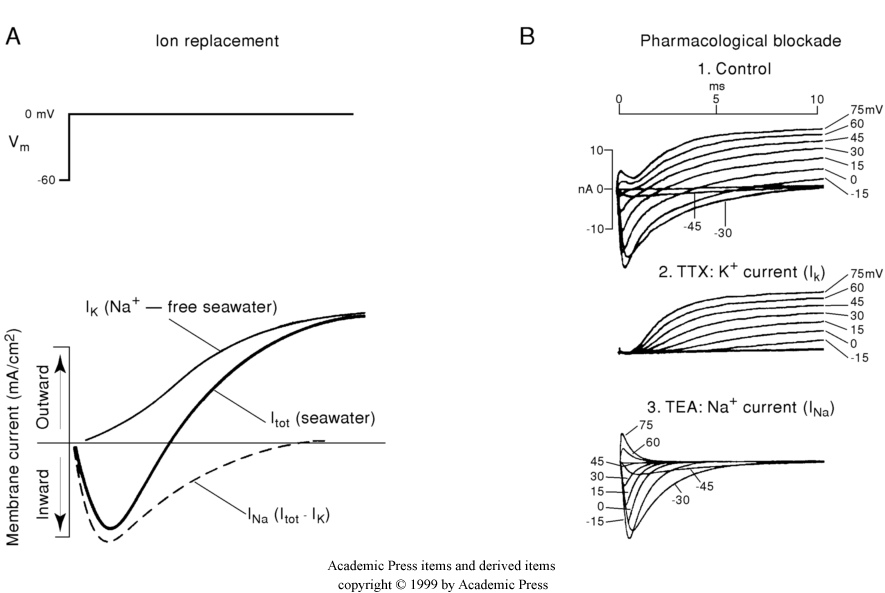
\includegraphics[width=\textwidth]{pharmacological-blockade.png}
\item Voltage dependent conductance for $g_{Na}, g_{K}$
\subitem No static voltage
\item Action potential\\
\end{itemize}

\begin{figure}[H]
        \centering
        \begin{subfigure}[b]{0.6\textwidth}
                \centering
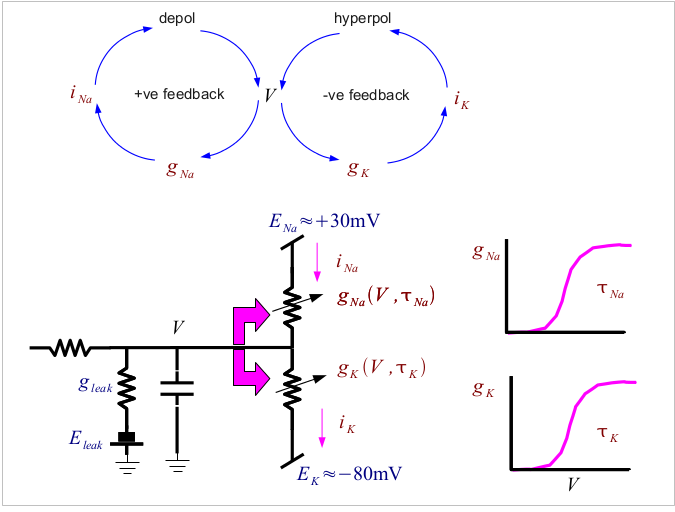
\includegraphics[width=\textwidth]{pos-neg-feedback-loops.png}
        \end{subfigure}%
        ~
        \begin{subfigure}[b]{0.4\textwidth}
                \centering
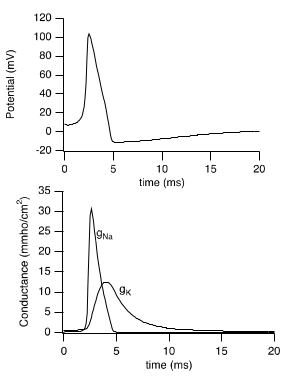
\includegraphics[width=\textwidth]{action-potential.png}
        \end{subfigure}
\end{figure}

\begin{itemize}
\item $g_{Na}$ increases quickly, but then inactivation kicks in and it decreases again.
\item $g_K$ increases more slowly, and only decreases once the voltage has decreased.
\item The $Na^+$ current is autocatalytic. An increase
in V increases g, which increases the $Na^+$
current, which increases V, etc.
\item The threshold for action potential
initiation is where the inward $Na^+$ current
exactly balances the outward $K^+$ current.\\
$\rightarrow g_{Na} > g_K $(leads to the spike[depolarisation]) $\rightarrow g_{K}$ increases $ b                                                                         \rightarrow g_{K} > g_{Na} $(hyperpolarisation)\\
\end{itemize}

\subsection{The Hodgkin-Huxley equations}
$C\frac{dV}{dt} + \bar{g}_{K}n^4 (V-V_K)+\bar{g}_{Na}m^3 h(V-V_{Na})+\bar{g}_L(V-V_L) + I_{injected} = 0$\\
\textbf{$m^3,n^4$} are part of the proposed model.\\
$\bar{g}_L(V-V_L)$ is the general leak.
\begin{itemize}
\item Both amplitude of conductance change and its time const g change with $V_{clamp}$
\item The m and n gates open with depolarisation
\item The h gate closes with depolarization\\
$\rightarrow$ Not symmetrical power (circuit currents),ap goes into one direction
\end{itemize}

\subsection{Saltatory conductance}
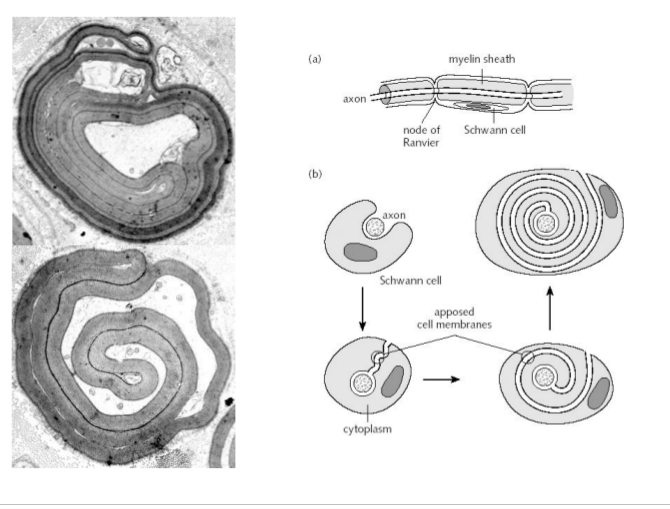
\includegraphics[width=0.7\textwidth]{myelinized-axons.png}
\begin{itemize}
\item Ranviernodes 
\item Myelinized by gliacells $\rightarrow$ resistance high/not leaking
\item The thicker the cell the faster the signal
\end{itemize}

\section{Lecture 5 - Synapse 1 (Rodney Douglas)}
\begin{itemize}
\item Neurotransmitter
\subitem Glutamat = excitation
\subitem GABA = inhibition
\item Synaptic mechanism
\subitem 1. Synthesis: Building blocks of transmitter substance are imported into the terminal where the neurotransmitter is synthesized and packaged into vesicles.
\subitem 2. Release: In response to an AP, the transmitter is released across the membrane by exocytosis.
\subitem 3. Receptor activation: The transmitter crosses the synaptic cleft and binds to a receptor.
\subitem 4. Inactivation: The transmitter is either taken back into the terminal or inactivated in the synaptic cleft.

\end{itemize}

\begin{figure}[h]
\begin{center}$
\begin{array}{cc}
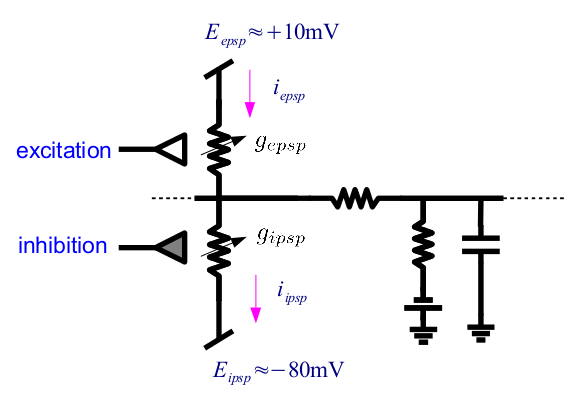
\includegraphics[width=0.5\textwidth]{ex-inhib-elec-membrane.png}
&
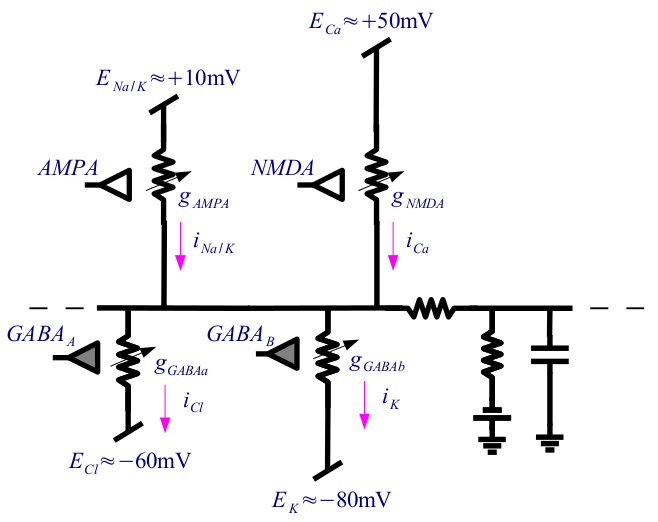
\includegraphics[width=0.5\textwidth]{AMPA-NMDA-GABA-elec-membrane.png}

\end{array}$
\end{center}
\end{figure}
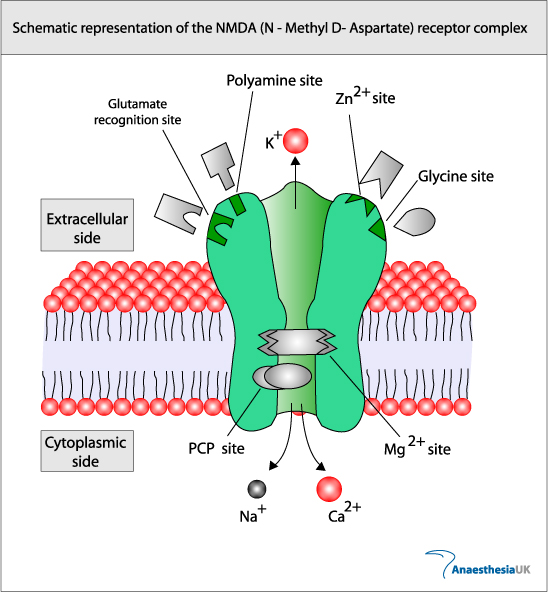
\includegraphics[width=0.5\textwidth]{nmda.png}

\subsection{Glutamate receptor}
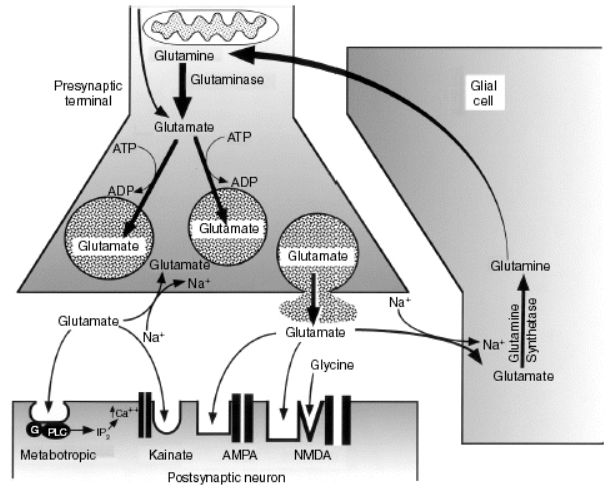
\includegraphics[width=0.7\textwidth]{glutamate-neuron.png}
\begin{itemize}
\item NMDA-receptor: Depolarization$\rightarrow MG^{2+}$ is removed. Activation by Glutamate and co-agonist $\to Ca^{2+}$ can float in\\
$\searrow Ca^{2+},Na^+,K^+$
\item AMPA-receptor: Calcium activates NMDA-receptor. Second messenger activates. Weak stimulation by Glutamate only AMPA receptor is bound to Glutamate.\\
$\searrow Na^+,K^+,Ca^{2+}$
\item Important feature of NMDA-receptor
\subitem Activation of glutamate requires co-agonists glycine or serine.
\subitem Effect requires coincidence of depolarization of post-synaptic membrane to dislodge $Mg^{2+}$ and binding of agonist.
\subitem Relatively slow post-synaptic EPSP
\subitem 10x more permeable to $Ca^{2+}$ than to $Na^+$ or $K^+$
\end{itemize}

\begin{tabular}{|l|l|l|l|l|l|}
\hline
Receptor & Transmitter & ion & Approx $E_{rev}$ & Agonist & Antagonist\\
\hline
AMPA & glutamate & Na, K, Ca & +0mV & AMPA & CNQX\\
\hline
	NMDA & glutamate & Ca, Na, K & +10mV & NMDA(glycine) & AP5,ketamine,MK-801\\
\hline
	mGLU & glutamate & G-coupled & & &\\
\hline
	 GABAa & gaba & Cl & -60mV & muscimol & bicuculine\\
\hline
	GABAb & gaba & K/G-coupled & -80mV & baclofen & saclofen\\
\hline
\end{tabular}

\section{Lecture 6 - Plasticity/Learning (Michael Pfeiffer)}

\subsection{Learning \& Memory}
\begin{itemize}
\item Learning is the acquisition of new information or knowledge
\item Memory is the retention of learned information
\item Types of memory
\subitem Declarative Memory (Facts,Events)
\subitem Non-Declarative Memory
\subitem Procedural Memory (Skills, Habits)
\subitem Emotional responses
\item Facts about Synapses
\subitem Neurons communicate via AP and are interconnected via synapses
\subitem Information is represented by distributed activity
\subitem Learning and memory is based on changes in synaptic connections(Formation \& retraction of synapses(development),Changes in synaptics efficacies(plasticity))
\end{itemize}

\subsection{Plasticity}
What is plasticity?\\
Axiomatic rule: Everything is somehow encoded in synapses.\\
No information in the shape of the spike, but in the frequency and synchronicity.\\
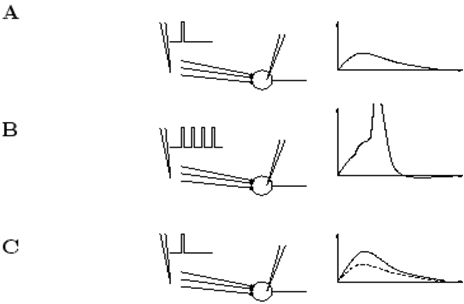
\includegraphics[width=0.8\textwidth]{plasticity.png}
\begin{itemize}
\item Modification of postsynaptic potentials (PSP) evoked by presynaptic spikes
\subitem A. Postsynaptic response triggered by a weak test pulse (left).
\subitem B. Strong stimulation sequence (left) triggers postsynaptic firing.
\subitem C. A later test pulse evokes a larger postsynaptic response than initially.
\item Parameters that define synapse strenghts
\subitem Neurotransmitter and receptor type
\subitem Position of synapse
\subitem Availability of vesicles
\subitem Re-uptake
\subitem Neuromodulators(Dopamin etc.)
\subitem „Non-synaptic“ plasticity(excitablity of neurons, dendritic branch strength)
\subitem Postsynaptic cellular processes
\subitem Pre-/postsynaptic firing
\subitem etc.
\item Diseases affect plasticity: Alzheimer, Parkinson
\end{itemize}

\subsection{Models of plasticity}
\begin{itemize}
\item Non-synaptic plasticity(Excitability of neurons, dendritic branch strength)
\item Synaptic plasticity
\subitem 1.Phenomenological models(High-level,relationships between activity \& plasticity etc. exp: Pavlov Classical conditioning)
\subitem 2.Biophysical models (Low-level,cellular processes etc. exp: Hebbian learning)
\end{itemize}
\subsection{Pavlovian Learning}

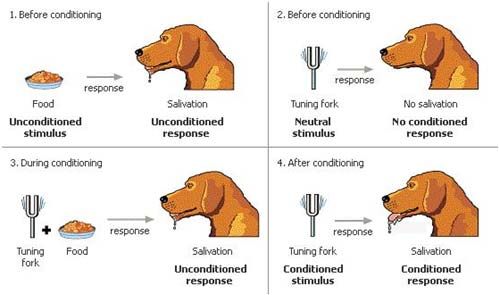
\includegraphics[width=0.8\textwidth]{pavlovian-conditioning.png}

\subsection{Hebbian Learning}
\begin{itemize}
\item "Fire together, wire together"
\item Learning based on correlations between pre- and postsynaptic firing
\item Uses only variables locally available at the synapse
\item Rate-based model: $\Delta synaptic-efficacy_{neuron A,neuron B} \propto firing-rate_{neuron A} \cdot firing-rate_{neuron B}$
\item Only weight increase modelled/No depression\\
$\rightarrow$ Can lead to instability (positive feedback loops)
\item Other rules: BCM rule, Oja's rule
\item Implications:
\subitem Global effects arise from local learning
\subitem Variables(pre- \& postsynaptic action potential,efficacy(weight),local concentration)
\end{itemize}

\subsection{NMDA synapse}
\begin{itemize}
\item Can act as coincidence detector for pre- and postsynaptic firing
\item Backpropagation action potentials
\item Depolarization from other synapses
\item Calcium influx crucial for plasticity
\item Strong NMDA activation $\rightarrow$ potentiation
\item Weak NMDA activation $\rightarrow$ depression
\end{itemize}

\subsection{Short term plasticity(STP)}
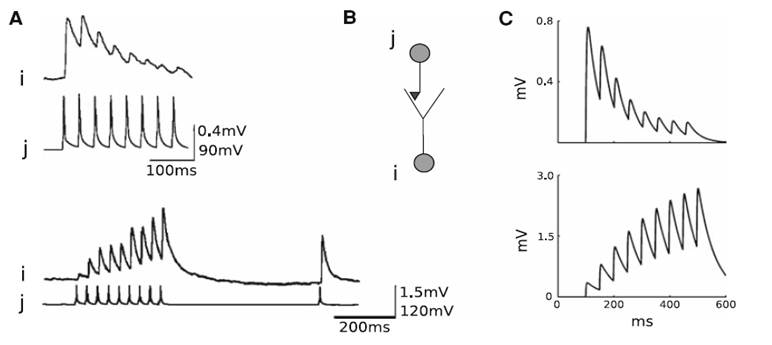
\includegraphics[width=0.8\textwidth]{STP.png}
\begin{itemize}
\item A neuron j fires several times, neuron i fires as well and the spike size is increased(the higher the spike, the more efficient the neuron), but decreases after a short time.(Caused by loss of vesicles)
\item Effect goes away in order of seconds.
\end{itemize}
\subsection{Long term plasticity(LTP)}
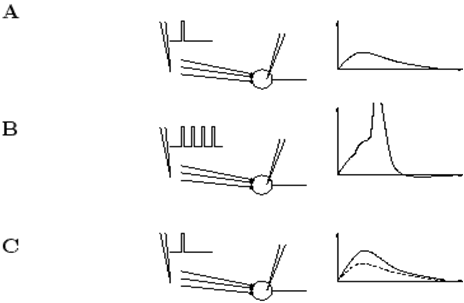
\includegraphics[width=0.8\textwidth]{LTP.png}
\begin{itemize}
\item Schematic drawing of a paradigm of LTP induction. \subitem A. A weak test pulse (left) evokes the postsynaptic response sketched on the right-hand side of the figure. 
\subitem B. A strong stimulation sequence (left) triggers postsynaptic firing (right, the peak of the action potential is out of bounds). 
\subitem C. A test pulse applied some time later evokes a larger postsynaptic response (right; solid line) than the initial response. The dashed line is a copy of the initial response in A. (schematic figure).
\item LTP occurs if a synapse and the post-synaptic neuron are simultaneously depolarized beyond a threshold. This can occur in cooperation (weak and weak or weak and strong signals)
\item 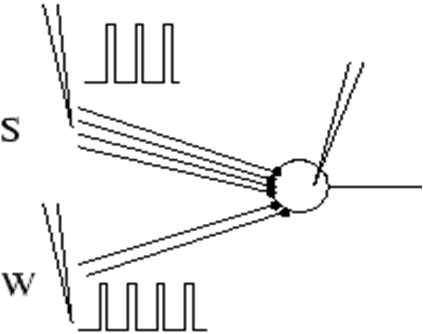
\includegraphics[width=0.5\textwidth]{LTP-coop.png}\\
Cooperativity in the induction of LTP. Weaker synapse W is strengthend if the postsynaptic neuron is active and both presynaptic sites are firing.
\end{itemize}

\subsection{Spike-timing dependent plasticity (STDP)}
\begin{itemize}
\item Not only correlation, but also timing of the spikes determines plasticity.
\item Sign of plasticity is determined by local calcium
concentration
\item Postsynaptic spike travels back to the dendritic tree and activates voltage-dependent Ca channels
\item Presynaptic activity can allow Ca influx through
NMDA channels (if postsynaptic part is sufficiently
depolarized)
\item If pre-spike is soon afterwards followed by post-
spike, NMDA-R activity is supralinearly enhanced by
depolarization due to backpropagating spike
$\rightarrow Ca^{2+}$ determines the strength of plasticity
\item Functional consequence:
\subitem Correlated firing groups win the battle against uncorrelated groups (depression). Battle of two correlated groups have a random winner.\\
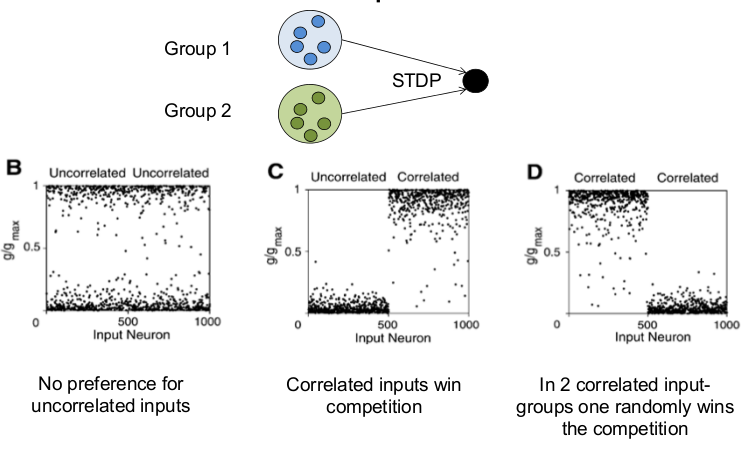
\includegraphics[width=0.8\textwidth]{STDP-consequences.png}
\end{itemize}

\subsection{Facts}
\begin{itemize}
\item A lot of diversity in STDP occurances
\item Different plasticity in different brain areas
\item Diversity of neuron and synapse types
\item Large number of control parameters for plasticity experiments (frequency, timing, postsynaptic voltage, position on the dendrite, ...)
\item Influence of neuromodulators, calcium, drugs, and various proteins
\item Long-term vs. short-term effects
\item It is unlikely that there is one single model that explains all plasticity effects found in biology
\end{itemize}

\subsection{Dopamine}
\begin{itemize}
\item Neurotransmitter and neuromodulator
\item Significant for motor processes (Parkinson),pleasure and reward, motivation, attention, emotions
\item DA activation is a relatively
homogeneous, global population signal
\item DA activation is related to rewarding stimuli or reward prediction errors
\item Reinforcement learning
\item Dopamine can extend
the timing window for LTP
\item Dopamine can convert LTD into LTP
\end{itemize}

\section{Lecture 7 - Perceptron Learning Algorithm}
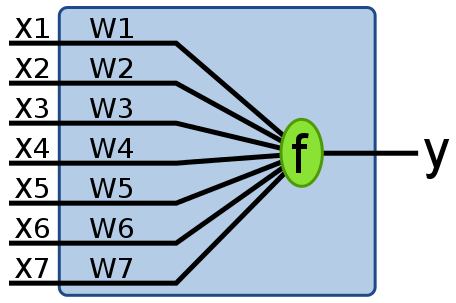
\includegraphics[width=0.4\textwidth]{perceptron.png}\\
Perceptron, McCulloch-Pitts Neuron, Linear Threshold Unit\\
\begin{itemize}
\item Model represents a neuron as a number of inputs X (dendrites) and one output Y (axon). The weights W determine the influence of a dendrite input, which is either exitatory or inhibitory. f is a function that defines how to combine the weights x and w(normally $\sum (w_i \cdot x_i)$) and $\theta$ (not shown in picture but usually at the place between y and f) is normally a bias that is added to the sum to compare the result to 0.
\item Each neuron has two states: active(1) \& inactive(0)
\item Summing up the products + the bias $\sum x_i\cdot w_i + bias$, then compared to 0 gives us either an ouput of 1 for sums $\ge 0$ or a 0 if < 0.
\item Using this model, we can create conventional electronic gates such as AND-Gate, OR-Gate and NOT-Gate. 
\item However the XOR-Gate/NXOR-Gate is not possible in this model. Both functions are not linear.
\item Similarities to biological neurons
\subitem Active or inactive state
\subitem Directionality(input/output)
\subitem Activity dependent of weighted functions of other neurons
\item Differences to biological neurons
\subitem Continous time vs. discrete time
\subitem Degrees of activation
\subitem Activation as a function of the inputs of a real neuron is not linear.
\end{itemize}

\subsection{Perceptron Learning Algorithm}
Given a set of (input vector$x_i$, desired output$d_i$) pairs, finds weights that produce the desired output$d_i$.(If such weights exist)\\
\begin{itemize}
\item Choose random weights
\item Calculate actual output.
\item $y_i = f[w(t)\cdot x_j] = \sum w_i \cdot x_i$ + bias
\item If wrong output $\rightarrow$ change weights
\item For every weight $w_i(t+1) = w_i(t) + \alpha(d_j-y_j(t))x_i$
\item This is repeated until the iteration error $\frac{1}{s}\sum_j^2[d_j-y_j(t)]$ is less than a user-specified error threshold $\gamma$ or until we completed a predefined numer of iteration.
\item Algorithm creates a sufficient result if a solution exists.
\end{itemize}

\section{Lecture 8 - Nervous System Organization(Kevan Mastin)}
\begin{itemize}
\item Brain consists of:
\subitem Spinal cord
\subitem Hindbrain
\subitem Midbrain - Thalamus
\subitem Forebrain - Neocortex, Hippocampus
\item Whitematter
\subitem Glia cells, myelinated axons
\item Greymatter
\subitem Neurons 
\end{itemize}

\begin{figure}[H]
        \centering
        \begin{subfigure}[b]{0.5\textwidth}
                \centering
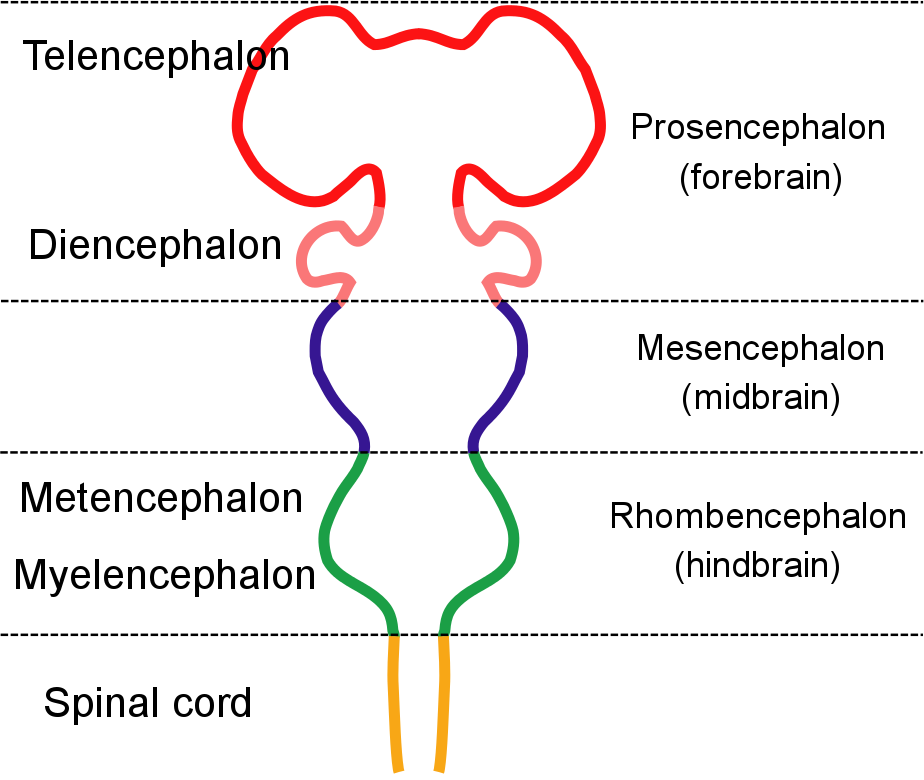
\includegraphics[width=\textwidth]{brain-parts.png}
        \end{subfigure}%
        ~
        \begin{subfigure}[b]{0.5\textwidth}
                \centering
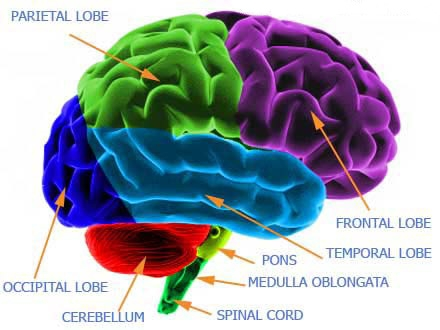
\includegraphics[width=\textwidth]{brain.png}
        \end{subfigure}
\end{figure}
\begin{figure}[H]
        \centering
        \begin{subfigure}[b]{0.5\textwidth}
                \centering
				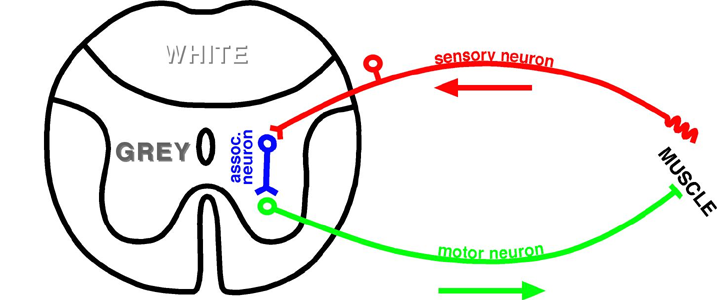
\includegraphics[width=\textwidth]{motor-sensory-neuron.png}
        \end{subfigure}%
        ~
        \begin{subfigure}[b]{0.5\textwidth}
                \centering
				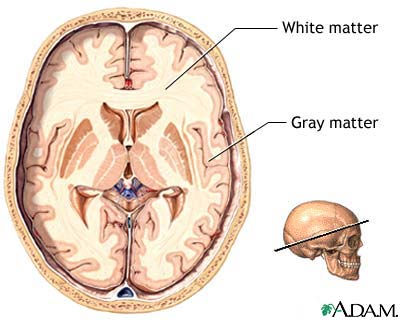
\includegraphics[width=\textwidth]{brain-cut.png}
        \end{subfigure}
\end{figure}
White matter $1mm^3\rightarrow$ 9m axons\\
Grey matter $1mm^3\rightarrow$ 50'000 neurons\\
$\rightarrow$ Long distance communication needs space

\section{Lecture 9 - Synapse 2(Kevan Mastin)}
\begin{itemize}
\item Sherrington (1873)
\subitem First research on synapses
\item Vagus nerve
\subitem Stimulating the vagus nerve slows down the heart beat $\rightarrow$ inhibitory function.
\item Synapse
\subitem Only vesicles which are already on the presynaptic membrane will be released after the AP (not all vesicles are released after an AP)
\subitem One single synapse produces only a small potential. it needs many synapses to create an actual AP. $\rightarrow$ Release of neurotransmitters is Ca dependent.
\item Probabilistic release of neurotransmitter
\subitem Presynaptic problem
\subitem All synapses have probabilistic release
\subitem Factors (\# of synapses, \# of postsynaptic receptors) = Plasticity
\end{itemize}

\section{Lecture 10 - Rate/Event Coding (Michael Pfeiffer)}
\begin{itemize}
\item What is neural coding?
\subitem How is information encoded?
\subitem Single neuron firing $\leftrightarrow$  Population firing
\subitem How does a neuron encode information?
\subitem Firing rate, Timing of spikes
\subitem What do different measurement techniques tell us about the neural code?
\subitem Spatial/temporal resolution
\subitem What is a useful visualization of firings for interpretation?
\begin{figure}[H]
        \centering
        \begin{subfigure}[b]{0.5\textwidth}
                \centering
				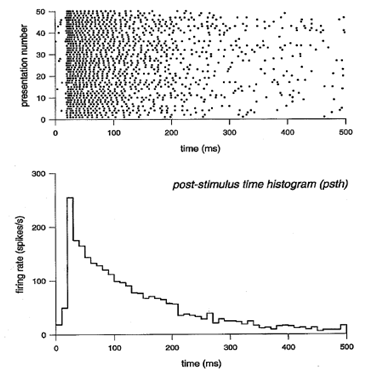
\includegraphics[width=\textwidth]{neural-coding-problem.png}
				\caption{Raster plot = spikes \& Histogram}
        \end{subfigure}%
        ~
        \begin{subfigure}[b]{0.5\textwidth}
                \centering
				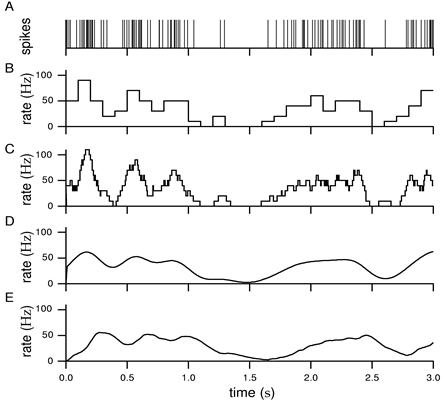
\includegraphics[width=\textwidth]{firing-rate.png}
				\caption{100ms time bins $\rightarrow$ 100ms sliding window $\rightarrow$ gauss filter $\rightarrow$ causal filter}
        \end{subfigure}
\end{figure}
\end{itemize}

\subsection{Neuronal rate codes(average over time(single neuron))}
\begin{itemize}
\item Tuning curves
\subitem 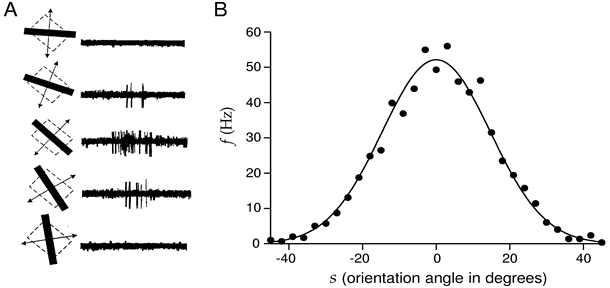
\includegraphics[width=0.9\textwidth]{tuning-curve.png}
\subitem Shown line and its response primary visual cortex. Turning curve shows average firing rate of varying stimulus parameters. Tuning curves characterize a single cell.\\
\subitem 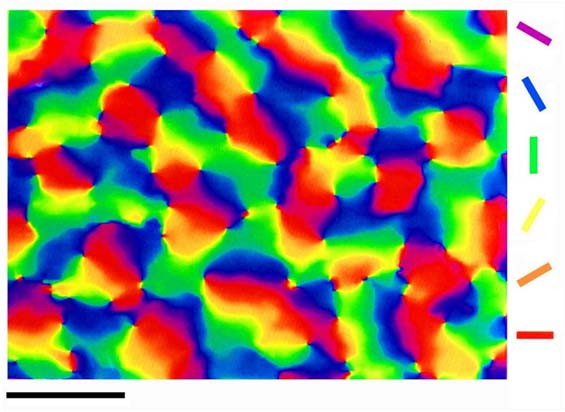
\includegraphics[width=0.7\textwidth]{orientation-map.png}\\
Nearby neurons have similar preferred orientations(colors)
\item Rate codes\\ + easy to understand\\ -No timing effects\\ -Might be misleading(More than one stimulus might be encoded)
\end{itemize}

\subsection{What can a single neuron encode?}
\begin{itemize}
\item Places(on entering a particular region)
\item Grids (regularly arranged triangular grid of locations)
\item Head-direction
\item Single cell responds to one single human face(''Grandmother cell'')
\end{itemize}

\subsection{Population rate(average over pool of equivalent neurons)}
\begin{itemize}
\item Population codes
\subitem Different cells encode different range of the stimulus $\rightarrow$ allows accurate reconstruction of the signal(sparse coding,exp. 3 types of color cones in retina)\\

\subitem Population vector code\\
Populations of neurons stand for vector directions, encoded direction is vectorial addition weighted by firing rate.\\

\subitem Neuronal Event codes\\
Time-to-first spike codes\\
-Can implement competition among different cells\\
-Can be rank-order code(sequence matters)

\subitem Burst- and Temporal Codes\\
Bushcricket auditory neurons in natural environment preserve very high coding precision in extreme noise\\
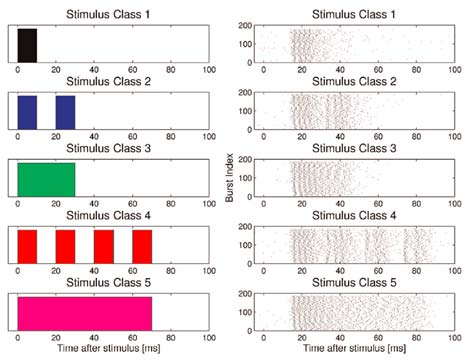
\includegraphics[width=0.7\textwidth]{burst-code.png}

\subitem Oscillations and Phase Coding\\
The neurons fire at different phases with respect to the background oscillation\\
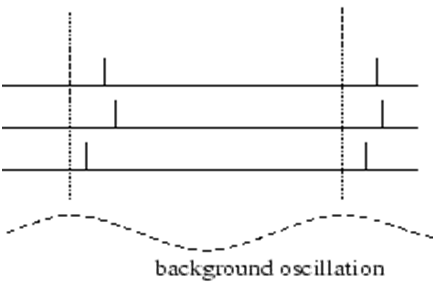
\includegraphics[width=0.6\textwidth]{phase-code.png}

\subitem Local Field Potential(LFP)\\
-Low-pass filtered extracellular recording\\
-Reflects the integration of membrane currents in a local region\\
-Dominated by dendritic synaptic activity\\
-Might encode different properties of the stimulus than single cell firing\\
-Where does it come from / what does it show?\\
-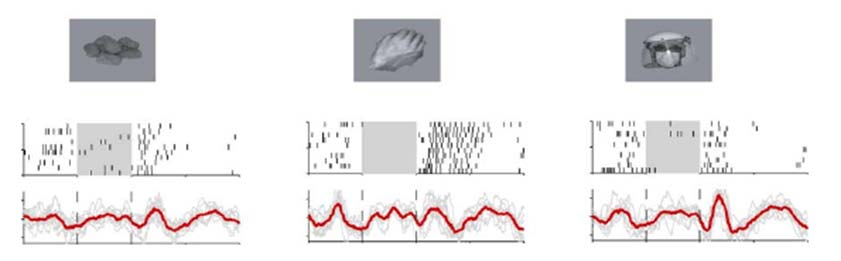
\includegraphics[width=\textwidth]{MUA-LFP.png}\\
MUA(upper signal) \& LFP (lower signal)
\subitem fMRI (functional magnetic resonance imaging)\\ based on blood oxygenation level
\subitem Synchrony coding\\
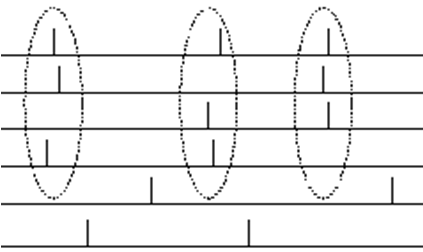
\includegraphics[width=0.6\textwidth]{synchrony-code.png}
\end{itemize}
\subsection{Binding problem}
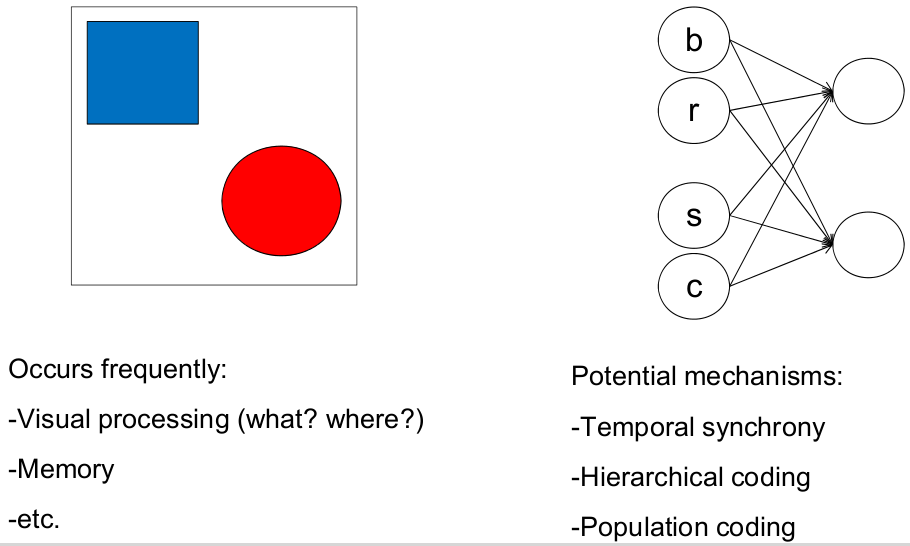
\includegraphics[width=0.9\textwidth]{binding-problem.png}
\subsection{Averages \& Estimation}
\begin{itemize}
\item Spike Triggered Average
\begin{figure}[H]
        \centering
        \begin{subfigure}[b]{0.5\textwidth}
                \centering
				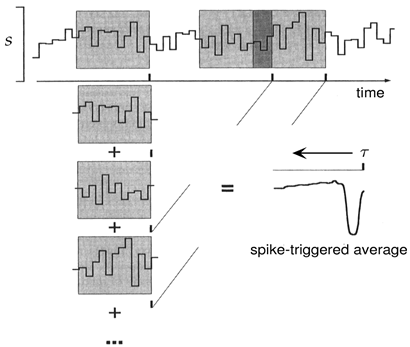
\includegraphics[width=\textwidth]{spike-triggered-average.png}
				\caption{Average over stimulus in short time window before spike}
        \end{subfigure}%
        ~
        \begin{subfigure}[b]{0.5\textwidth}
                \centering
				\includegraphics[width=\textwidth]{stimulus-estimation.png}
				\caption{Stimulus estimation}
        \end{subfigure}
\end{figure}
\item Issues to remember:
\subitem Whole stimulus reconstruction may not be relevant
\subitem Evolution may have shaped us to encode particular features better than others (e.g. faces)
\subitem Cells may respond to only particular aspects of stimulus
\subitem Cells may respond to multiple aspects of stimulus
\subitem Artificial stimuli used for studies may be predictable
\end{itemize}

\section{Lecture 11 - Hopfield Networks(Matthew Cook)}

\begin{itemize}
\item In a hopfield network, every node is connected to every other node(One single layer of nodes). The network of nodes is in some state at any time. Some of the states are stable and some are not. The nodes are connected by edges with weights and each node holds a value of -1/1 or 0/1. While the network is not in a stable state, updating the network leads to a state change that ultimately converges to a certain stable state (local minimum). The update of the nodes can be done synchronous or asynchronous over the nodes.\\
\item Synchronous updates yields a stable pattern or a cycle of 2 patterns.
\item Asynchronous updates are done with a greedy min-cut algorithm.
\item When we update a node,we consider weights to that node from all other active nodes.
\item If the sum of all weights of the active nodes is higher than zero then this neuron is active too.\\
\includegraphics[width=0.7\textwidth]{hopfield-network.png}\\
Update function:
$a_{i,t}$ = output of unit at time t\\
$a_{i,t+1} =
\left\{
	\begin{array}{ll}
		1   & \sum_{j=1}^N a_{i,t}\cdot w_{ij} > \theta_i (\mbox{often 0}) \\
		-1 & \mbox{otherwise}
	\end{array}
\right.$
\end{itemize}

Features:\\
A hopfield network is an associative type of memory just as the human memory and is able to remember states it learned before. A Hopfield network of 100 nodes can store about approximately 15 pictures(stored as local minima in the network or stable states). Important is that the pictures are distinct, otherwise it can be that the network gets new stable states and the pictures only get ''half remembered''.\\
\includegraphics[width=0.4\textwidth]{hopfield-network-face-recog.png}

\section{Lecture 12 - Feed-Forward Networks(Matthew Cook))}
\begin{itemize}
\item Feed-Forward Network with back-propagation is a network that is single-directed(multiple layers of nodes) and has a certain number of inputs x and a certain number of outputs f. Every layer of nodes ''feeds'' the next layer with information.
\item In many applications the nodes use a sigmoid function as an activation function.
\item Back-propagation is a way method that lets information flow backwards inside of the single directed network, but that seems not the way biology is doing it. It is a learning technique that compares the output values $f_i$ to the desired values $g_i$ to compute corrective values with a predefined error function.\\
$E = \sum (f_i -g_i)^2$

\item The error is then propagated back through the network to adjust the weights of each connection to reduce the deviation from the desired values. The network will converge to either no or just a small error.
\item To adjust weights properly, one optimizes by a method called gradient descent:\\
$\frac{\delta E}{\delta w_k} = \sum 2(f_i - g_i) \cdot \frac{\delta(f_i - g_i}{\delta w_k} = \sum 2(f_i - g_i) \frac{\delta f_i}{\delta w_k}$
\item Feed inputs to network one at a time. Compare output to desired output $f_i - g_i$
\item For each weight, compute the sensitivity of output $\frac{\delta f_i}{\delta w_k}$
\item Adjust weights $w_k$ by $\epsilon \cdot (f_i - g_i) \frac{\delta f_i}{\delta w_k}$


\end{itemize}

\section{Lecture 13 - Interacting Neural Populations(Matthew Cook)}

Population codes\\
Idea: Information is represented by the pattern of activity in a neural population. Specially, neurons are ''tuned'' to preferred stimuli.\\
\begin{itemize}
\item We train a monkey to hold its gaze fixed while we move a visual stimulus around. The monkey holds its gaze fixed at E = \colorbox{magenta}{$-15^\circ$}/\colorbox{green}{$0^\circ$}/\colorbox{blue}{$15^\circ$}(eye angle) while we move the stimulus from R =$-40^\circ ... 40^\circ$ (retinal angle).
\end{itemize}

\begin{figure}[H]
        \centering
        \begin{subfigure}[b]{0.3\textwidth}
                \centering
\includegraphics[width=\textwidth]{one-cell-tuning-curve.png}
                \caption{Tuning curve of one cell}
        \end{subfigure}%
        ~
        \begin{subfigure}[b]{0.3\textwidth}
                \centering
\includegraphics[width=\textwidth]{cell-order.png}
                \caption{Cells ordered by response to $20^\circ$}
        \end{subfigure}
        ~ 
        \begin{subfigure}[b]{0.3\textwidth}
                \centering
				\includegraphics[width=\textwidth]{3D-visualisation.png}
                \caption{3D visualization of cell's response to different degrees}
        \end{subfigure}
\end{figure}

\begin{figure}[H]
        \centering
        \begin{subfigure}[b]{0.5\textwidth}
                \centering
\includegraphics[width=\textwidth]{ape-picture.png}
                \caption{Monkey holding gaze fixed on point $10^\circ$ and light falling in from $20^\circ$}
        \end{subfigure}%
        ~
        \begin{subfigure}[b]{0.5\textwidth}
                \centering
				\includegraphics[width=\textwidth]{Retina-Eye-Auditory.png}
                \caption{Visualization of Retina angle ordering cell set R, Eye angle ordering set E,2D result population C and auditory direction set A.}
        \end{subfigure}
\end{figure}

\begin{figure}[H]
        \centering
        \begin{subfigure}[b]{0.3\textwidth}
                \centering
				\includegraphics[width=\textwidth]{Cell-A.png}
                \caption{Cell A $\in$ R}
        \end{subfigure}%
        ~
        \begin{subfigure}[b]{0.3\textwidth}
                \centering
				\includegraphics[width=\textwidth]{Cell-B.png}
                \caption{Cell B $\in$ A}
        \end{subfigure}
        ~ 
        \begin{subfigure}[b]{0.3\textwidth}
                \centering
                \includegraphics[width=\textwidth]{Cell-C.png}
				\caption{Cell C $\in$ E}
        \end{subfigure}
\end{figure}

\begin{figure}[H]
        \centering
        \begin{subfigure}[b]{0.3\textwidth}
                \centering
				\includegraphics[width=\textwidth]{Cell-D.png}
                \caption{Cell D $\in$ C}
        \end{subfigure}%
        ~
        \begin{subfigure}[b]{0.3\textwidth}
                \centering
				\includegraphics[width=\textwidth]{Cell-E.png}
                \caption{Cell E (Not every neuron shows clear tuning curves)}
        \end{subfigure}
\end{figure}

\section{Lecture 14 - Neuromorphic VLSI(Giacomo Indiveri)}
\subsection{VLSI}
\begin{itemize}
\item Very Large Scale Integration Technology allows us to fabricate chips and memories. Digital VLSI( Today's computers) not analog, not low power, not fault tolerant, not robust to inhomogeneities, not asynchronous (clocked), not massively parallel
\item Neuromorphic = VLSI systems containing electronic analog/digital circuits that exploit the physics of silicon to reproduce the bio-physics of neural circuits present in the nervous system. Two main goals:
\subitem To understand the computational properties of biological neural systems using standard CMOS VLSI technology as a tool.
\subitem To exploit the known properties of biological systems to design and implement efficient devices for engineering applications.
\item Neuromorphic VLSI neuron circuits
\subitem To reproduce the physics of neural computation using subthreshold analog circuits and asynchronous digital circuits.
\subitem To build autonomous learning behaving systems that can interact with the environment in real–time
\end{itemize}

\subsection{Why VLSI for neural computation?}
\begin{itemize}
\item Best exploit current and future VLSI technologies
\item Optimally suited for nano- and future emerging technologies
\item Ideal tools for real- and accelerated-time modeling of neural systems
\item Compact, low-power sensory processing devices for autonomous/flying robots, embedded systems, etc.
\item Direct interface to living systems
\end{itemize}

\subsection{Different remarkable circuits}
\begin{itemize}
\item Artificial neuron model by McCulloch \& Pitts
\item Integrate \& fire model (I\&F)
\item
\begin{figure}[H]
        \centering
        \begin{subfigure}[b]{0.5\textwidth}
                \centering
\includegraphics[width=\textwidth]{conductance-based-SI-neuron.png}
                \caption{Conductance-based silicon neuron}
        \end{subfigure}%
        ~
        \begin{subfigure}[b]{0.5\textwidth}
                \centering
				\includegraphics[width=\textwidth]{axon-hillock-circuit.png}
                \caption{Axon-Hillock-circuit}
        \end{subfigure}
\end{figure}
\begin{figure}[H]
        \centering
        \begin{subfigure}[b]{0.5\textwidth}
                \centering
\includegraphics[width=\textwidth]{IanF-circuit.png}
                \caption{Ultra low-power generalized I\& F circuit}
        \end{subfigure}%
        ~
        \begin{subfigure}[b]{0.5\textwidth}
                \centering
\includegraphics[width=\textwidth]{multineuron-circuit.png}
                \caption{Spiking multineuron architectures}
        \end{subfigure}
\end{figure}
\end{itemize}
\end{document}
